\spread{Does a plausible alternative help identify the answer?}
\noindent An occupation and a birthplace can both be prominent on a biographical page. We tested whether the reader could identify which one the question asked for by comparing the plausible answers with one another.
\platehere{Figure_179_alternative_visual_answers}{A change in the selected evidence can change the meaning of a reply}{In \textbf{a}, the story question asks how the king felt. Both answers borrow the wording of the question and neither gives the feeling. In \textbf{b}, the first two readers answer the birthplace question with Dinant, Belgium. The competing reader gives the subject's academic post. These are original stopped replies. The story panel uses the first difference that fits the display. The Chinese panel uses the first exact loss that fits, after searching for an exact gain. The earlier signed reader and writer remained frozen.}
\begin{multicols}{2}
\section*{The competing evidence}
The same reader proposes up to 32 locations in the page image for each pictured question. The new model represents a location by its two endpoints and the mean state of its interior. In the independent control, a query attends to these three states. In the competing model, it can also attend to all the other proposed locations. Both fits add 57,984 trainable parameters and begin with the same scores. The writer receives the pictured question and one selected strip. It generates the reply freely.
\section*{A controlled change of preference}
Let $u_i$ be the score when attention is confined to the candidate, and $d_i$ the change when rivals become visible. Candidate $i$ can strictly overtake $j$ precisely when $d_i-d_j>u_j-u_i$. If the original winning margin exceeds $2\max_i|d_i|$, its winner is preserved. Lean checks these arithmetic statements under integer scoring. We checked the margin on the actual floating-point scores. Removing rival attention changed 21 of 192 Chinese examination strips. Adding it gained two exact strips and lost one. On 92 story questions it changed four strips, with no change in the four exact selections. Reversing candidate order changed scores by less than $10^{-5}$.
\section*{Training and transfer}
Of 39,057 original training questions, 32,387 had an annotated answer among the proposed locations. Both arms made eight passes on these lists. Constructing the shared bank used 1.71 kJ on one RTX 4090 D; the independent and competing fits used 0.94 and 0.87 kJ. Together with the parent reader and writer, each deployed system contains 1,135,306 parameters. Both matched zero of 128 held long answers and zero of 68 conversational replies. Neither retrieved a requested historical specimen in 260 tests.
\section*{Learning from a complete answer}
Let $p_s$ be the probability of selecting strip $s$ and $L_s$ the frozen writer's probability of an accepted stopped reply given that strip. Distinct accepted image streams are disjoint events. Their total likelihood induces the posterior $q_s=p_sL_s/\sum_j p_jL_j$. The gradient of negative log answer likelihood with respect to a selector logit is $p_s-q_s$. Thus a complete human answer can teach a selector even if it never occurs as a strip. We checked 2,848 strip--wording combinations on 64 questions from distinct training stories. On 53, no strip matched a reference. All 53 supplied a nonzero gradient. This numerical result tests the training signal; generalization requires fitting parameters and asking new questions.
\end{multicols}
\newpage
\spread{What can the writer say with its best possible evidence?}
\noindent We tested 862 questions on 431 new pages. The narrative questions have educator-written answers and come from 46 held FairytaleQA stories. Each pair asks about the same pictured section.
\platehere{Figure_180_writing_after_candidate_comparison}{Evidence training and autonomous answers}{\textbf{a}, Exact stopped replies on new Chinese examination, English narrative, English and Chinese MLQA, and English DROP questions. The narrative cohort has 92 questions, the others 192 each. One additional English statement pair survived the exclusions and is reported separately. \textbf{b}, Mean negative log likelihood of annotated locations per supported training list. Training loss fell in both arms.}
\begin{multicols}{2}
\section*{Free answers}
The independent and competing scorers respectively wrote 61 and 56 exact Chinese examination replies, and 17 and 15 exact Chinese MLQA replies. Both wrote zero exact narrative replies. An automated, anonymized meaning assessment on the same 80 questions gave 20 credits to the independent scorer, 17 to the competing scorer, 17 to the parent and 55 to Qwen3-VL 8B Q4. The Qwen3 8B judge saw two opposite candidate orders. Its human and sibling-answer controls passed calibration on each cohort. These scores include short factual answers and paraphrases.
\section*{An upper bound from the actual writer}
We fed every distinct candidate strip to the unchanged writer. Across 476 questions this produced 14,967 distinct question--strip inputs and reproduced all 476 originally selected replies. Some candidate yielded a complete exact answer on 139 of 192 new Chinese exam questions, 38 of 192 earlier English statement questions and none of 92 new story questions. On the first 16 story questions, at least one stopped reply received semantic credit on nine. The same panel procedure credited the chosen reply on two. Multiple comparisons allow a permissive judge more chances to accept a weak reply. Only 12 questions passed both controls on every panel; six of those had a credited candidate.
\end{multicols}
\begin{center}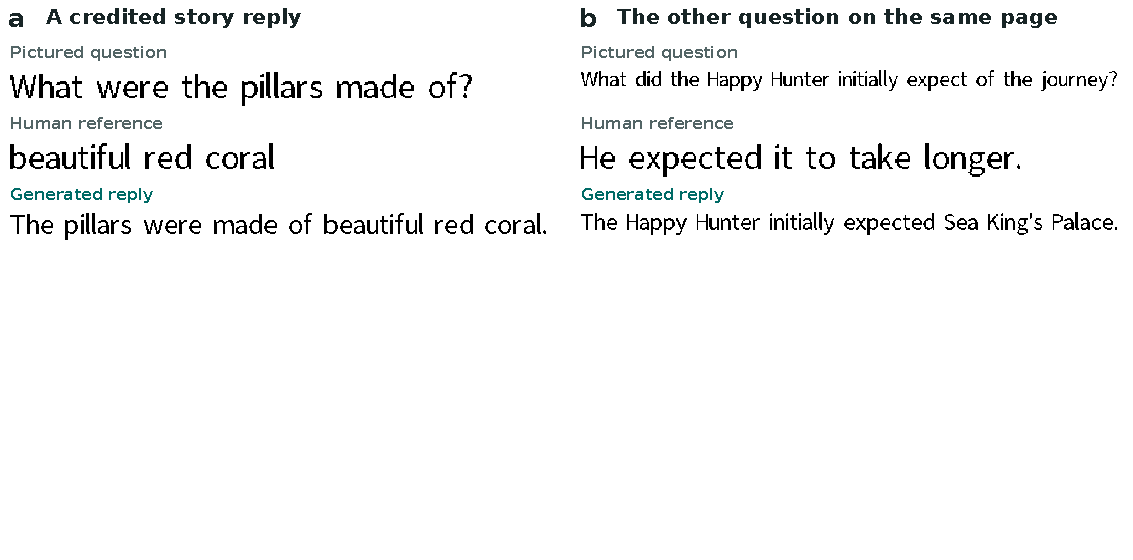
\includegraphics[width=.9\linewidth,trim=0 145bp 0 0,clip]{../figures/Figure_181_two_questions_in_a_story.pdf}\end{center}
\noindent{\small\textbf{Asking twice about one story.} First narrative question credited in both orders of the primary assessment, with its paired question. The writer names the material of the pillars. Asked about the expected duration of a journey, it gives a destination. Both outputs use the same page. Story data from Xu et al., \href{https://aclanthology.org/2022.acl-long.34/}{FairytaleQA}.}
\newpage
